\documentclass[12pt, a4paper]{report}

\usepackage{graphicx} % For including images
\usepackage{hyperref} % For clickable hyperlinks
\usepackage[utf8]{inputenc} % For UTF-8 encoding
\usepackage{imakeidx} % For the index

\makeindex % Command to make an index

\begin{document}

% Title Page
\title{Your Thesis Title}
\author{Your Name}
\date{\today}
\maketitle

% Abstract
\begin{abstract}
  This is the abstract of your thesis. Write a brief summary of the content here.
\end{abstract}

% Table of Contents
\tableofcontents

% Index Page
\printindex

\chapter{Introduction}
\label{chap:introduction}
This is the introduction chapter.\index{Introduction}

% Adding a figure
\begin{figure}[h!]
  \centering
  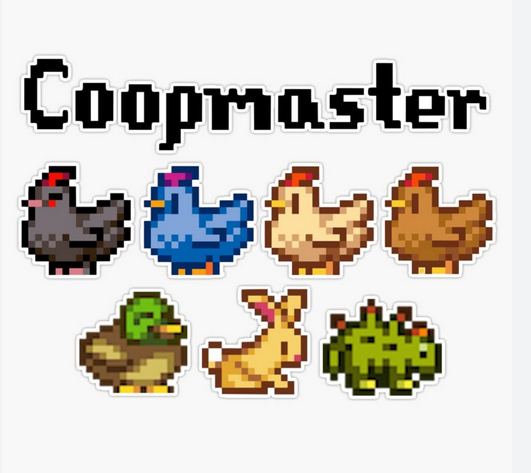
\includegraphics[width=0.8\textwidth]{./images/coopmaster}
  \caption{An example image.}
  \label{fig:example}
\end{figure}

\chapter{Literature Review}
\label{chap:literature}
This chapter covers the literature review.\index{Literature}

% Mermaid Charts
% You cannot natively include Mermaid diagrams directly in LaTeX without converting them first.

\chapter{Methodology}
\label{chap:methodology}
Description of the methodology used.\index{Methodology}

\chapter{Results}
\label{chap:results}
Presentation of results.\index{Results}

% References
\bibliographystyle{plain}
\bibliography{references} % references.bib should contain your bibliography

\end{document}
